\documentclass{article}
\usepackage{graphicx} 
\usepackage{wallpaper}
\usepackage{pgfgantt}
\usepackage{fancyhdr}
\usepackage{geometry}

\begin{document}


\begin{figure}
    \centering
    
\includegraphics[width=0.5\textwidth]{UC_V_FundoClaro-negro.eps}
\end{figure}
\linespread{2}
\title{\textbf{ \Huge GeoSciences Project}} 
\author{ Guilherme Miguel Machado de Matos Cruz \and João Antunes Celorico Ferreira da Piedade}

\date{October 2023}



\maketitle
\newpage
\linespread{1}
\section{Project Goal}
Provide to Earth Sciences Department of University of Coimbra the possibility to obtain and then analyse the soil humidity in diverse locations.

\section{Brief Description of our Project}
Our project aims to create a product capable of delivering reliable data to the Earth Sciences Department in our University so they can use that data to carry with several studies of how the rain affects the level of the water on ground-waters. This data will be taken by soil humidity sensors, connected with an ESP. The data will be uploaded to a SQL database, created by ourselves and visible in a Website created in HTML and CSS and hosted in a BlueHost domain.

\section{List of necessary materials}
\begin{itemize}
    \item Esp32 with an external connection to an WiFi antenna;
    \item Omni Direction Antenna FIT0505;
    \item 2x Water Proof Humidity Sensor SEN0308;
    \item Water Proof Cables.
\end{itemize}
\section{MoSCoW Analysis}
\textbf{Must Have:} \begin{itemize}
    \item Collect data from the humidity sensors;
    \item Upload the data to an SQL Database;
\end{itemize}
\textbf{Should Have:} \begin{itemize}
    \item Integrated Website that shows the live (every hour) data of the soil humidity;
    \item Low-key data analysis to delete "trash" data that, for some reason, were miscollected;
\end{itemize}
\textbf{Could Have:} \begin{itemize}
    \item Charts on the Website with the data;
    \item Data analysis to the collected data, such as average soil humidity on different zones, for example.
\end{itemize}
\textbf{Will Not Have} \begin{itemize}
    \item Predictive Analysis of the data;
    \item Integration with rain sensor on site.
\end{itemize}
\newpage
\newgeometry{top=2cm, bottom=3cm}

\section{Gantt Chart}


\begin{figure}[!htb]
\hspace*{-80px}% manually adjusted
  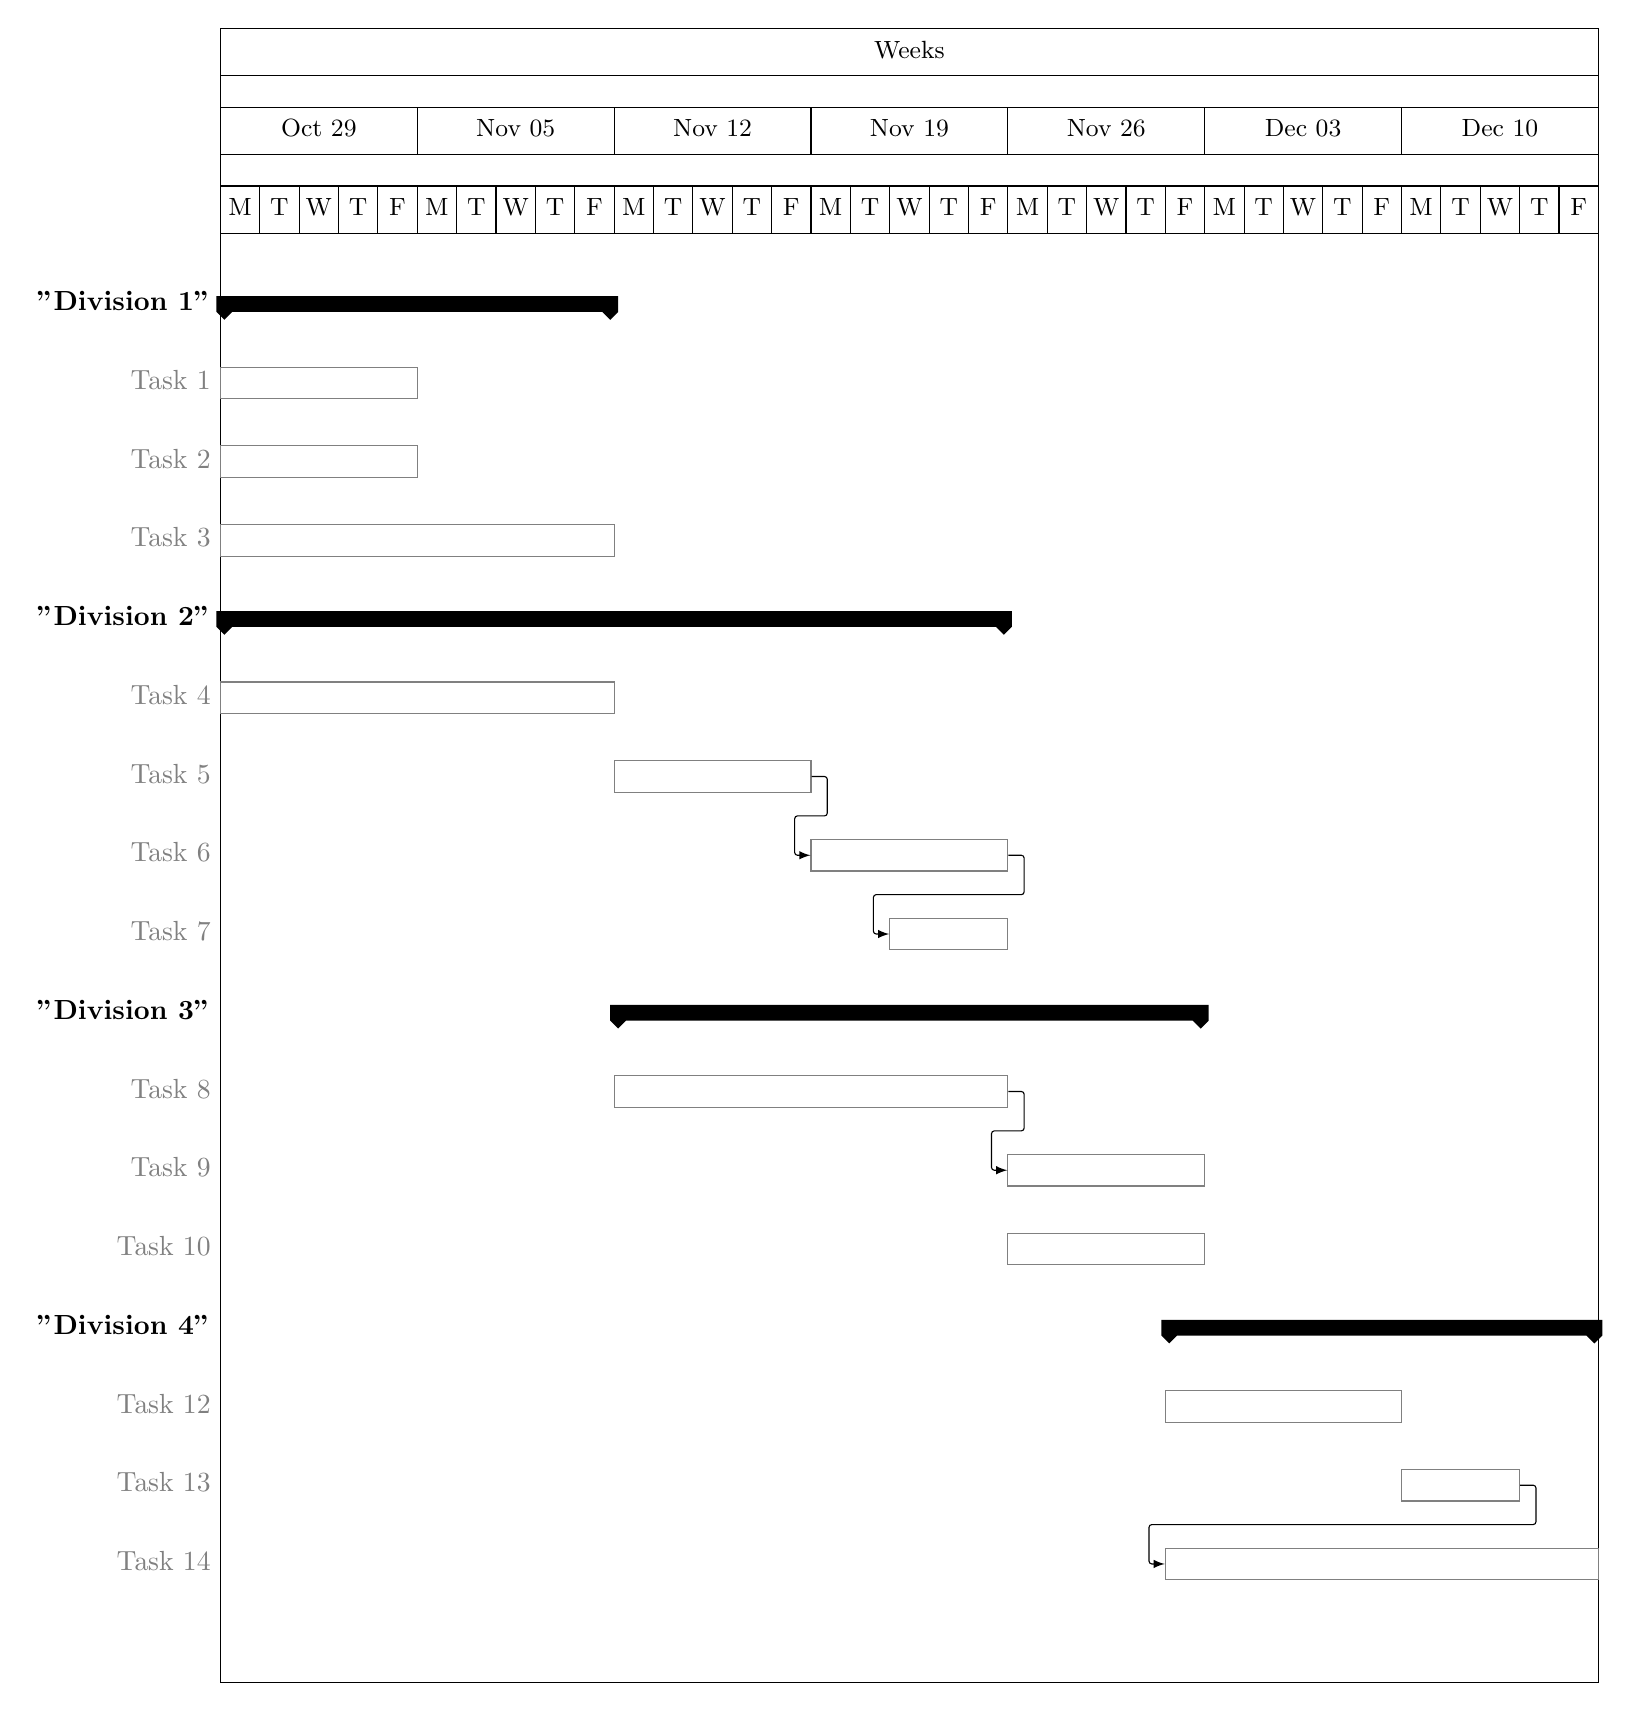
\begin{tikzpicture}

    \begin{ganttchart}{1}{35}
  \gantttitle{}{0} % Empty title for alignment
  \gantttitle{Weeks}{35} \\ % Subtitle above the year
  \gantttitlelist{"Oct 29", "Nov 05", "Nov 12", "Nov 19", "Nov 26", "Dec 03", "Dec 10"}{5}
  \ganttnewline
  \gantttitlelist{"M", "T", "W", "T", "F", "M", "T", "W", "T", "F", "M", "T", "W", "T", "F", "M", "T", "W", "T", "F", "M", "T", "W", "T", "F", "M", "T", "W", "T", "F", "M", "T", "W", "T", "F"}{1} \\
  \ganttgroup{"Division 1"}{1}{10} \\
  \color{gray}\ganttbar{Task 1}{1}{5} \\
  \ganttbar{Task 2}{1}{5} \ganttnewline
  \ganttbar{Task 3}{1}{10} \\
  \color{black}\ganttgroup{"Division 2"}{1}{20}\\
  \color{gray}\ganttbar{Task 4}{1}{10} \\
  \ganttbar{Task 5}{11}{15} \ganttnewline
  \ganttbar{Task 6}{16}{20} \\
  \ganttbar{Task 7}{18}{20} \\
  \color{black}\ganttgroup{"Division 3"}{11}{25}\\
  \color{gray}\ganttbar{Task 8}{11}{20} \\
  \ganttbar{Task 9}{21}{25} \ganttnewline
  \ganttbar{Task 10}{21}{25} \\
  \color{black}\ganttgroup{"Division 4"}{25}{35}\\
  \color{gray}\ganttbar{Task 12}{25}{30} \\
  \ganttbar{Task 13}{31}{33} \ganttnewline
  \ganttbar{Task 14}{25}{35} \\
  \color{black}\ganttlink{elem6}{elem7}
  \ganttlink{elem7}{elem8}
  \ganttlink{elem10}{elem11}
  \ganttlink{elem15}{elem16}
\end{ganttchart}  
  \end{tikzpicture}
\end{figure}
\restoregeometry



\title{\textbf{Caption of Gantt Chart}} \hfill \break
\begin{itemize}
    \item Division 1 - \textbf{Bureaucratic Work}
    \begin{itemize}
        \item Task 1- Update The Trello;
        \item Task 2 - Finish the Preliminary Report;
        \item Task 3 - Gantt Chart;
    \end{itemize}
    \item Division 2 - \textbf{Programming The Hardware}
    \begin{itemize}
        \item Task 4 - Create an SQL Database;
        \item Task 5- Connect the Sensors;
        \item Task 6 - Upload the Data to the SQL;
        \item Task 7 - Do some data verification;
    \end{itemize}
    \item Division 3 - \textbf{Software Development}
    \begin{itemize}
        \item Task 8- Create an HTML Website;
        \item Task 9 - Upload the data from the SQL to the Website;
        \item Task 10 - Host the Website in a GITHUB domain;
    \end{itemize}
    \item Division 4 - \textbf{Project Defense}
    \begin{itemize}
        \item Task 11- Edit the Video to present;
        \item Task 12 - Create an PPT presentation;
        \item Task 13 - Prepare the defense.
    \end{itemize}
    
\end{itemize}
\vfill{Made in \LaTeX}


\end{document}
